\documentclass[11pt]{article}
\usepackage[utf8]{inputenc}
\usepackage{amsmath, amssymb, amsthm}
\usepackage{graphicx}
\usepackage{hyperref}
\usepackage{enumitem}
\usepackage{booktabs}
\usepackage{geometry}
\geometry{margin=1in}

\title{Fictitious Play and Reinforcement Learning for Computing Equilibria in Repeated Zero-Sum Games}
\author{Ioannis Kasionis \and Ioannis Koutsoukis}
\date{\today}

\begin{document}

\maketitle

\section{Introduction}
The computation of equilibria in games is a central problem in game theory and multi-agent systems. Repeated zero-sum games, where the gain of one player is exactly balanced by the loss of the other, provide an ideal test-bed for studying learning dynamics in adversarial settings. In this work, we explore iterative learning algorithms that allow players to converge toward equilibrium strategies without requiring complete analytical solutions. We focus on comparing Fictitious Play (FP) with reinforcement learning (RL) methods—including Q-Learning, Minimax RL, and Belief-Based approaches—in two well-known games: Rock-Paper-Scissors and Matching Pennies.

\section{Theoretical Background}

\subsection{Repeated Zero-Sum Games}
Repeated zero-sum games consist of a stage game that is played over several episodes. In each round, both players select actions simultaneously. The payoff for one player is the negative of the other player's payoff, ensuring that the total payoff sums to zero. The repetition of the game allows players to learn from past outcomes, adapt their strategies, and potentially converge to a Nash equilibrium or a minimax solution. These games serve as a foundational model for adversarial interactions in economics, security, and machine learning.

\subsection{Learning Agents}
Several learning algorithms have been proposed to compute equilibria in repeated games:
\begin{itemize}
    \item \textbf{Fictitious Play (FP):} Players assume that opponents will play according to the empirical frequency of their past actions. They then choose the best response to these beliefs.
    \item \textbf{Q-Learning (QL):} An RL method where agents learn the expected utility of actions using a Q–table and update it iteratively via temporal difference learning.
    \item \textbf{Minimax RL:} A variation of Q–Learning adapted for adversarial settings, where agents aim to maximize the minimum gain against a worst-case opponent.
    \item \textbf{Belief-Based Methods:} Agents update probabilistic beliefs about the opponent's actions and choose their best response accordingly.
\end{itemize}

\section{Implementation}

\subsection{Environment Setup}
Two game environments were implemented in Python:
\begin{itemize}
    \item \textbf{Stochastic Rock-Paper-Scissors (RPS):} In this environment, the game is played in two states with different payoff matrices. A state transition function introduces stochasticity, altering the stage game dynamically.
    \item \textbf{Matching Pennies (MP):} A non-stochastic repeated zero-sum game with a fixed payoff matrix, where the payoff for one player is the negative of the other.
\end{itemize}
Each environment is encapsulated within a Python class that defines the state, payoff matrices, and state transition rules.

\subsection{Experimental Design}
Experiments were conducted by pitting every pair of the four agents (FP, QL, Minimax RL, Belief-Based) against each other in both game environments. For each experiment, multiple trials were executed, each spanning thousands of episodes. During these simulations, various performance metrics were recorded, including:
\begin{itemize}
    \item Moving average rewards.
    \item Cumulative scores over episodes.
    \item Q–value evolution and convergence.
    \item Policy evolution and learning stability.
    \item Joint action frequency.
\end{itemize}
The simulation results were exported to CSV files and subsequently visualized using an interactive Python Dash dashboard.

\section{Results \& Discussion}
\label{sec:results-discussion}

This section presents our experimental findings for two zero-sum games: 
Rock--Paper--Scissors (RPS) and Matching Pennies (MP). We analyze each 
pairwise agent matchup with respect to policy evolution, joint action 
frequencies, Q-value convergence, and cumulative scores. Figures 
throughout this section illustrate how different learning algorithms 
adapt and either converge to equilibrium play or systematically exploit 
an opponent.

\subsection{Rock--Paper--Scissors (RPS)}

\paragraph{Q-Value Convergence.}
Rock--Paper--Scissors is a zero-sum game with a well-known mixed-strategy 
Nash equilibrium (each action with probability $1/3$). 
Figures~\ref{fig:rps-minimax-convergence} and~\ref{fig:rps-ql-convergence} 
compare the norm difference between successive Q-tables for 
Minimax RL and Q-Learning, respectively. Minimax RL quickly drives the 
difference to near-zero, indicating stable Q-values. Q-Learning, however, 
shows persistent fluctuations (a higher, noisy baseline), suggesting it 
is continually adapting to a non-stationary opponent rather than 
converging to a fixed solution.

\begin{figure}[htbp]
    \centering
    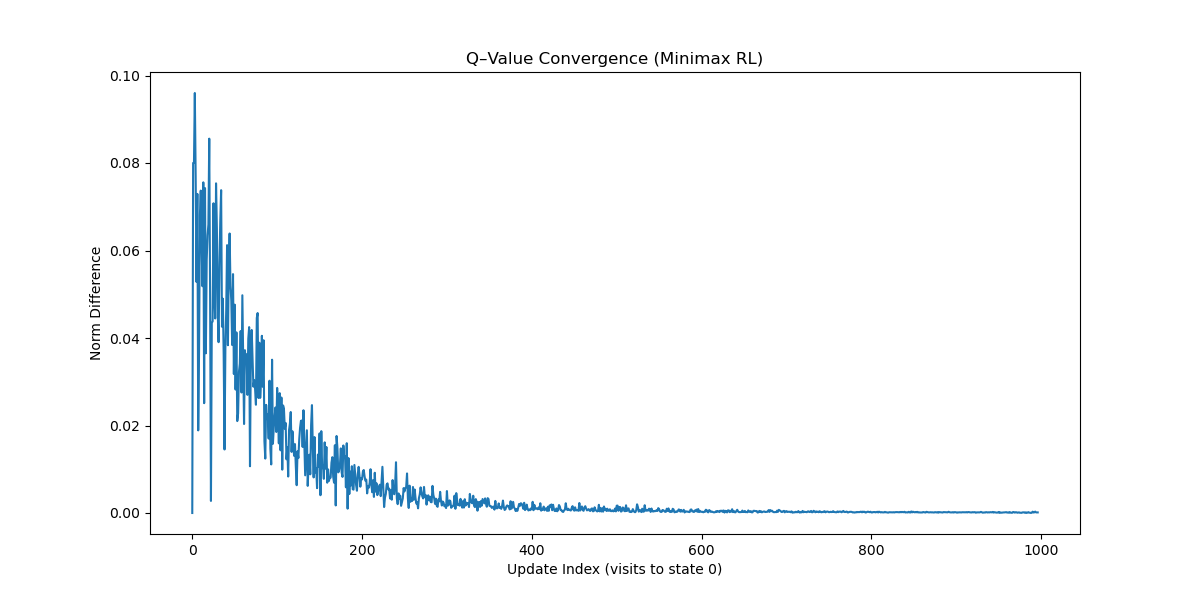
\includegraphics[width=0.6\textwidth]{rps-plots/ql_vs_mm_minimax_rl_qvalue_convergence.png}
    \caption{Q-Value Convergence for Minimax RL in RPS. The norm difference 
    quickly drops to near-zero, reflecting fast convergence to an 
    approximate equilibrium policy.}
    \label{fig:rps-minimax-convergence}
\end{figure}

\begin{figure}[htbp]
    \centering
    \includegraphics[width=0.6\textwidth]{rps-plots/ql_vs_mm_q-learning_qvalue_convergence.png}
    \caption{Q-Value Convergence for Q-Learning in RPS. The norm difference 
    remains noisy and never fully settles, as Q-Learning continuously 
    chases the opponent's changing strategy.}
    \label{fig:rps-ql-convergence}
\end{figure}

\paragraph{Policy Evolution and Joint Action Frequencies.}
Figure~\ref{fig:rps-fp-policy} shows how a Fictitious Play (FP) agent's 
action probabilities evolve over time. In many trials, FP ends up near 
the $1/3$-$1/3$-$1/3$ distribution, consistent with the RPS equilibrium. 
Joint action frequency heatmaps 
(e.g., Figure~\ref{fig:rps-joint-heatmap}) reveal that, for well-adapting 
agents, each of the nine possible (Rock, Paper, Scissors) combinations 
occurs with probability close to $1/9 \approx 0.11$. Small deviations 
reflect finite sample effects, exploration, or local biases.

\begin{figure}[htbp]
    \centering
    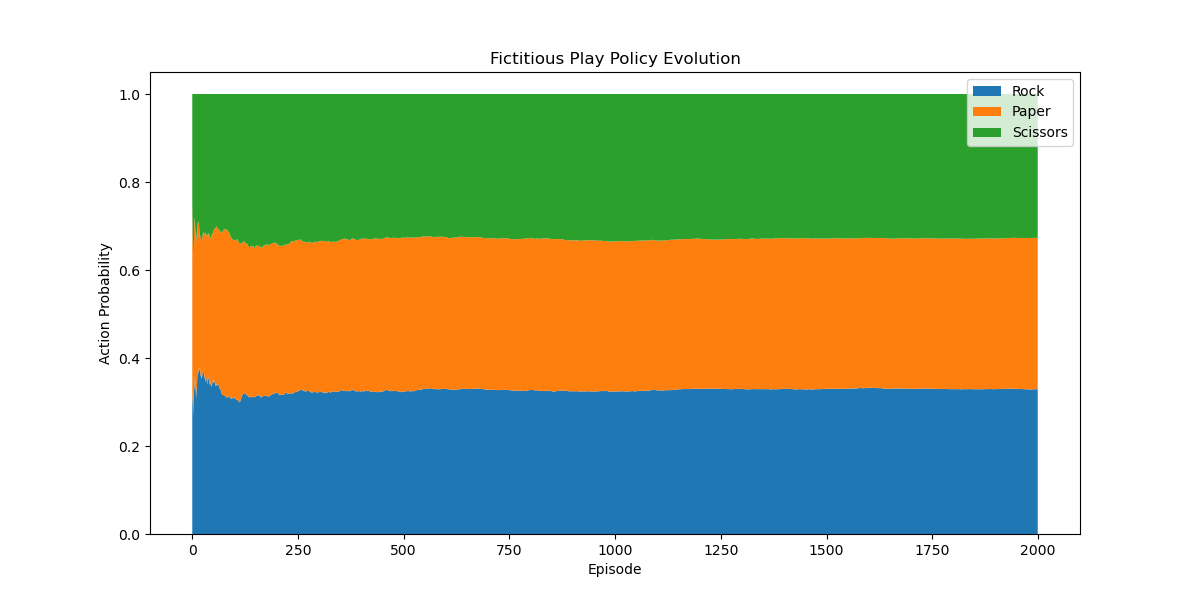
\includegraphics[width=0.6\textwidth]{rps-plots/fp_vs_mm_fictitious_play_policy_evolution.png}
    \caption{Fictitious Play policy evolution in RPS, showing action 
    probabilities for Rock, Paper, and Scissors. The agent often converges 
    near an even mix (one-third each).}
    \label{fig:rps-fp-policy}
\end{figure}

\begin{figure}[htbp]
    \centering
    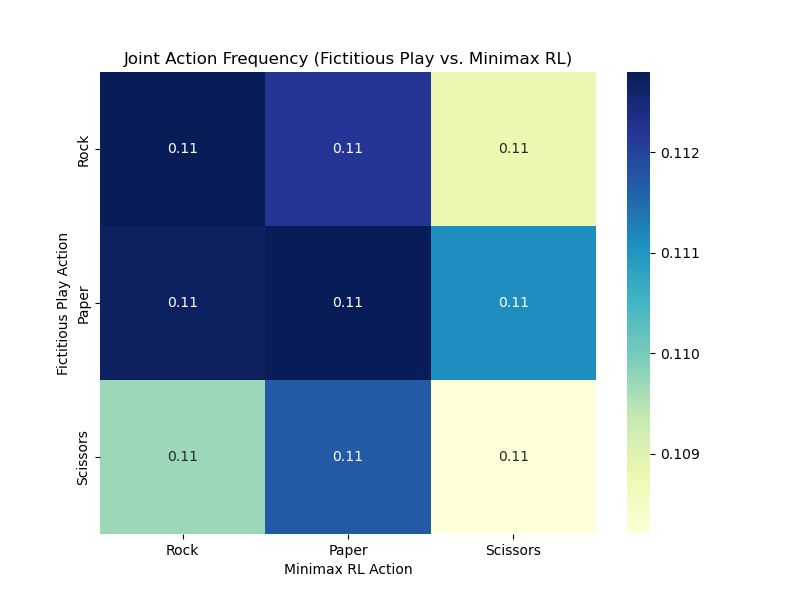
\includegraphics[width=0.6\textwidth]{rps-plots/fp_vs_mm_joint_actions.png}
    \caption{Joint Action Frequency for a pairwise matchup in RPS. Each 
    cell indicates how often (Action$_{A}$, Action$_{B}$) occurs. 
    Probabilities around 0.11 per cell suggest near-uniform randomization.}
    \label{fig:rps-joint-heatmap}
\end{figure}

\paragraph{Cumulative Scores.}
Figure~\ref{fig:rps-fp-mm-cumulative} shows sample cumulative score traces 
for different matchups. Some pairs (e.g., Minimax RL vs.\ Fictitious Play) 
hover around zero or oscillate, indicating near-equilibrium play. Others 
(e.g., Q-Learning vs.\ Belief-Based) exhibit diverging lines, meaning one 
agent exploits the other over time. Such divergences imply that one 
agent discovered a predictable bias in the opponent's actions and 
adapted to exploit it Figure~\ref{fig:rps-ql-bb-cumulative}.

\begin{figure}[htbp]
    \centering
    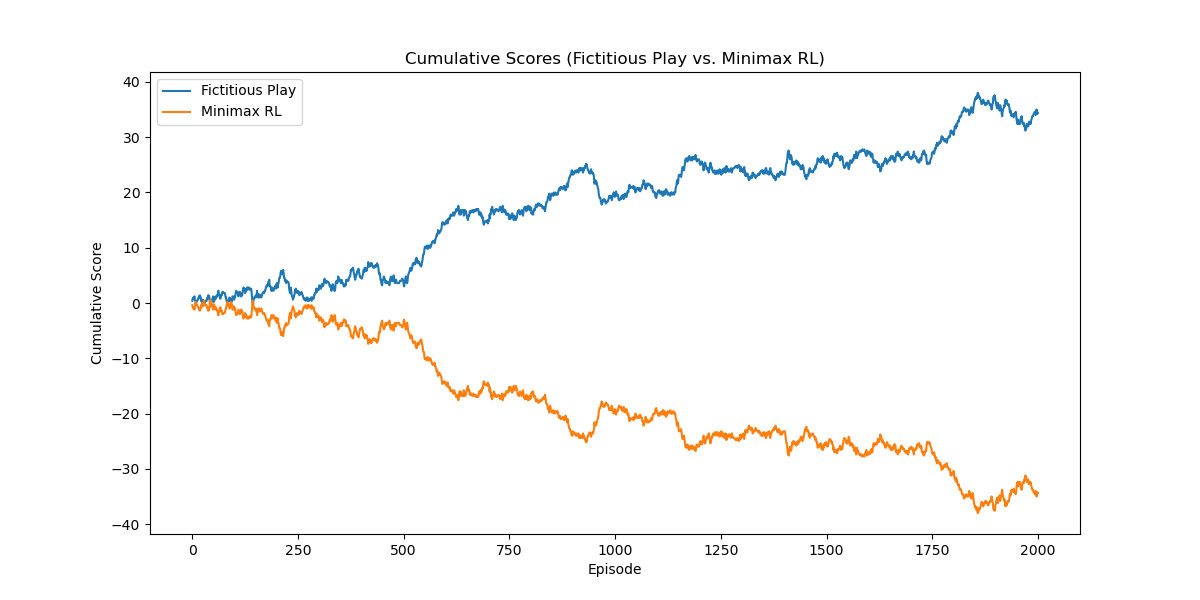
\includegraphics[width=0.6\textwidth]{rps-plots/fp_vs_mm_cumulative.png}
    \caption{Representative cumulative score evolution in RPS. When both 
    agents learn robust mixed strategies, scores fluctuate near zero. 
    Monotonic divergence implies one agent systematically exploits the other.}
    \label{fig:rps-fp-mm-cumulative}
\end{figure}

\begin{figure}[htbp]
    \centering
    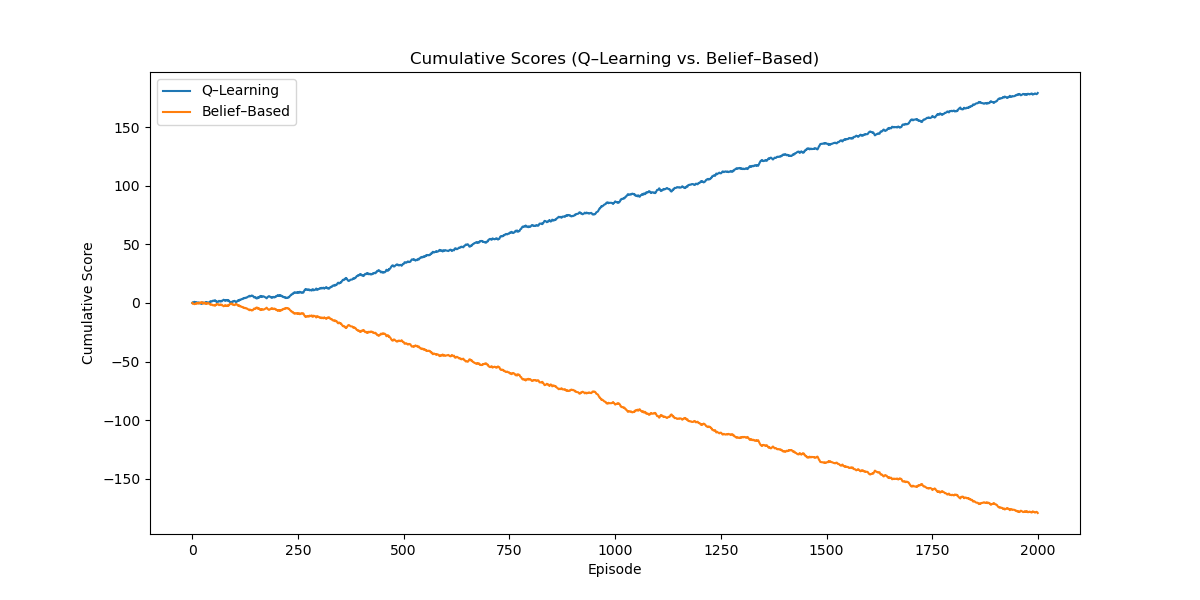
\includegraphics[width=0.6\textwidth]{rps-plots/ql_vs_bp_cumulative.png}
    \caption{Representative cumulative score evolution in RPS. When one 
    agent exploits the other over time. Such divergences imply that one 
    agent discovered a predictable bias in the opponent's actions and 
    adapted to exploit it.}
    \label{fig:rps-ql-bb-cumulative}
\end{figure}

\subsection{Matching Pennies (MP)}

Matching Pennies is another strictly competitive, zero-sum game but with 
only two actions: Heads or Tails. The unique Nash equilibrium requires 
each player to randomize 50--50.

\paragraph{Q-Value Convergence.}
Figures~\ref{fig:mp-minimax-convergence} and~\ref{fig:mp-ql-convergence} 
again contrast Minimax RL vs.\ Q-Learning. Minimax RL converges quickly 
to stable Q-values, while Q-Learning shows persistent norm-difference 
oscillations. As in RPS, Q-Learning's inability to account for a 
non-stationary opponent prevents it from ``locking in'' a stable solution.

\begin{figure}[htbp]
    \centering
    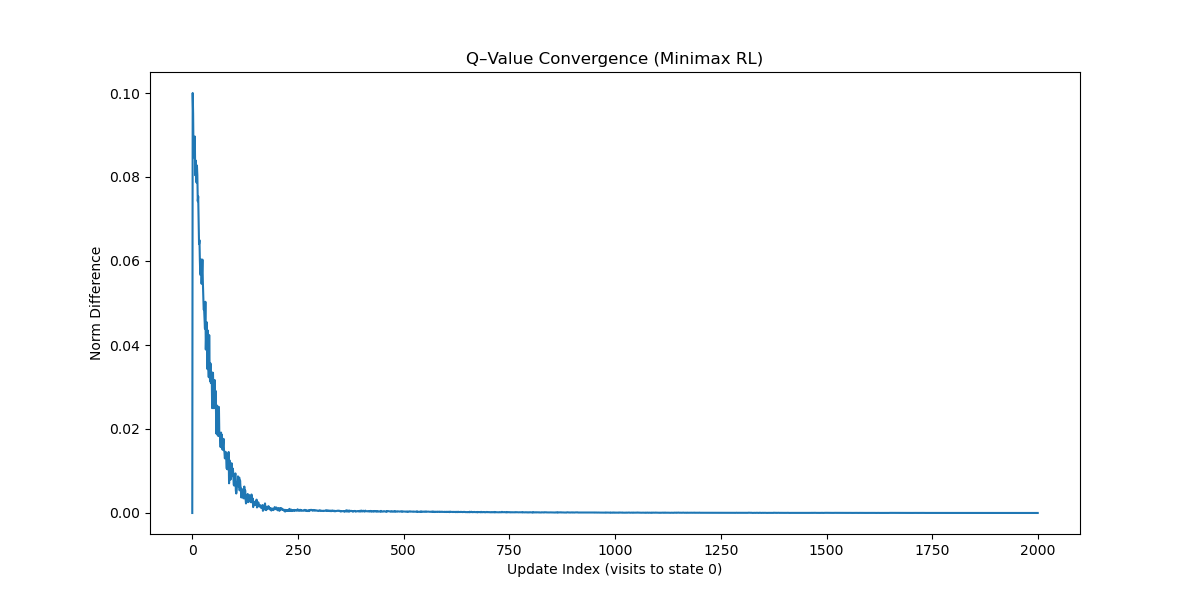
\includegraphics[width=0.6\textwidth]{mp-plots/ql_vs_mm_minimax_rl_qvalue_convergence.png}
    \caption{Q-Value Convergence for Minimax RL in Matching Pennies. The 
    agent rapidly converges to an approximate 50--50 strategy.}
    \label{fig:mp-minimax-convergence}
\end{figure}

\begin{figure}[htbp]
    \centering
    \includegraphics[width=0.6\textwidth]{mp-plots/ql_vs_mm_q-learning_qvalue_convergence.png}
    \caption{Q-Value Convergence for Q-Learning in Matching Pennies. 
    Norm differences remain higher and noisy, indicating ongoing 
    adaptation to the opponent's shifting policy.}
    \label{fig:mp-ql-convergence}
\end{figure}

\paragraph{Policy Evolution and Joint Frequencies.}
Figures like~\ref{fig:mp-fp-policy} show how Fictitious Play in 
Matching Pennies often approaches near 50--50 mixing if the opponent also 
mixes effectively. However, if an opponent remains predictably biased 
(e.g.\ Belief-Based with slow adaptation), Fictitious Play can lock in a 
counter‐bias, leading to a skewed distribution. Joint action frequency 
heatmaps, such as Figure~\ref{fig:mp-joint-heatmap}, reveal whether 
agents are truly randomizing (near 0.25 per cell in a 2$\times$2 
matchup) or getting stuck in more deterministic patterns.

\begin{figure}[htbp]
    \centering
    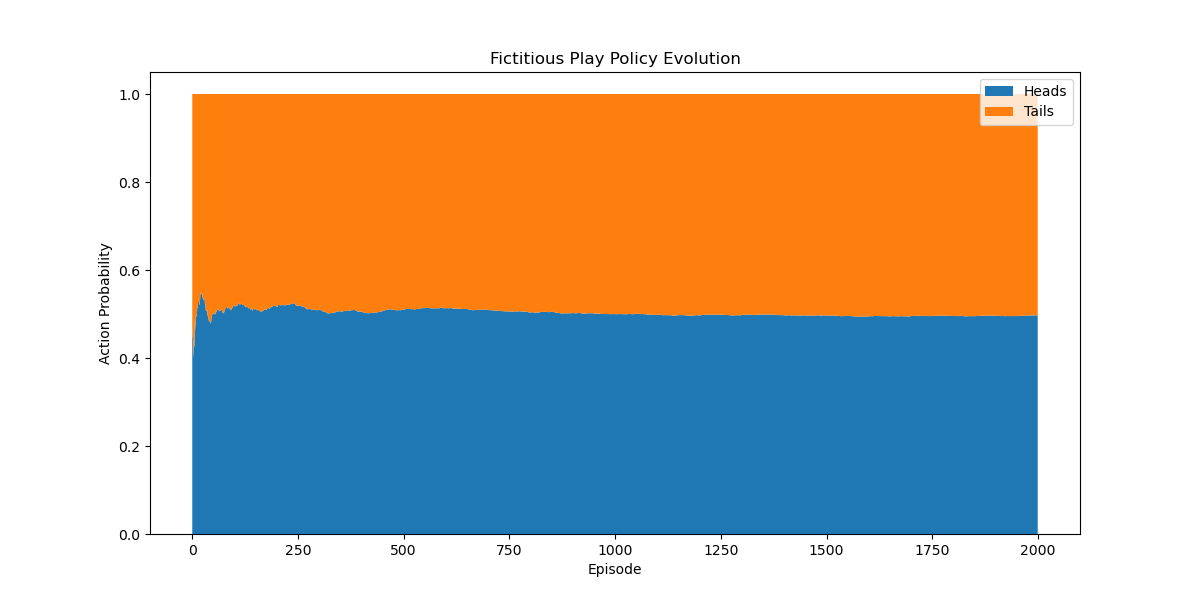
\includegraphics[width=0.6\textwidth]{mp-plots/fp_vs_mm_fictitious_play_policy_evolution.png}
    \caption{Fictitious Play policy evolution in Matching Pennies. 
    Equilibrium demands 50\% Heads and 50\% Tails, but slight 
    off-equilibrium biases can persist if the opponent remains 
    predictable.}
    \label{fig:mp-fp-policy}
\end{figure}

\begin{figure}[htbp]
    \centering
    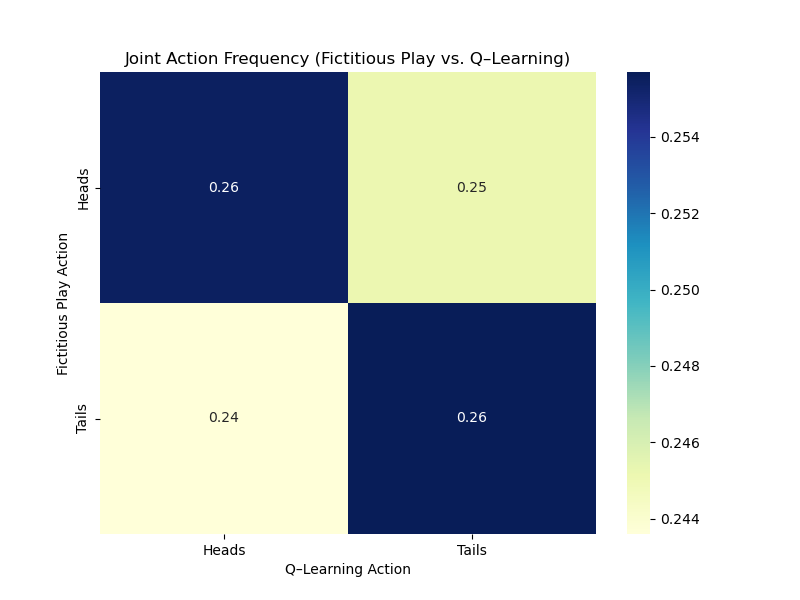
\includegraphics[width=0.6\textwidth]{mp-plots/fp_vs_ql_joint_actions.png}
    \caption{Joint Action Frequency in a 2$\times$2 (Heads/Tails) 
    matchup. Ideal equilibrium mixing would yield 0.25 in each cell. 
    Large deviations indicate that one or both agents are systematically 
    favoring certain actions.}
    \label{fig:mp-joint-heatmap}
\end{figure}

\paragraph{Cumulative Scores.}
Figure~\ref{fig:mp-ql-bb-cumulative} and Figure~\ref{fig:mp-fp-mm-cumulative} shows sample cumulative score traces in 
Matching Pennies. Because the game is strictly zero-sum, perfectly 
randomizing players would average zero. However, if one agent fails to 
correct a predictable pattern, the other agent’s cumulative score 
diverges positively while the former’s drops. For instance, Q-Learning 
often exploits slow‐adapting Belief-Based (resulting in a large positive 
slope), whereas Minimax RL vs.\ an adaptive agent might hover around 
zero or show moderate oscillations.

\begin{figure}[htbp]
    \centering
    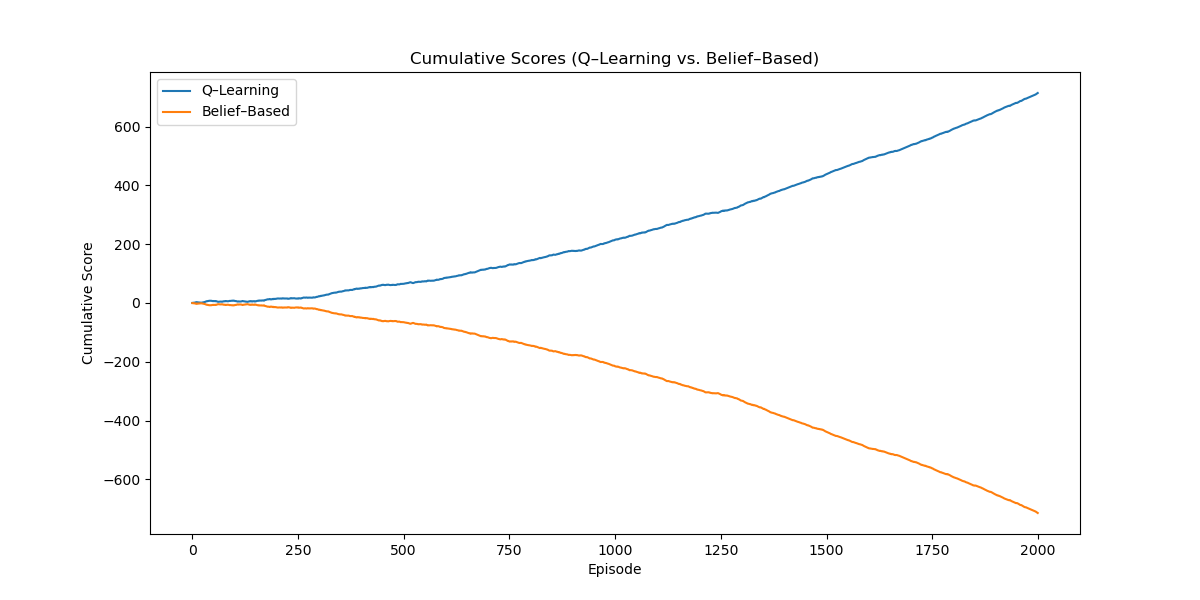
\includegraphics[width=0.6\textwidth]{mp-plots/ql_vs_bp_cumulative.png}
    \caption{Cumulative scores in Matching Pennies. Large, monotonic 
    separations imply one agent exploits the other's biased play. Near 
    zero or oscillatory outcomes suggest both agents approximate the 
    50--50 equilibrium.}
    \label{fig:mp-ql-bb-cumulative}
\end{figure}

\begin{figure}[htbp]
    \centering
    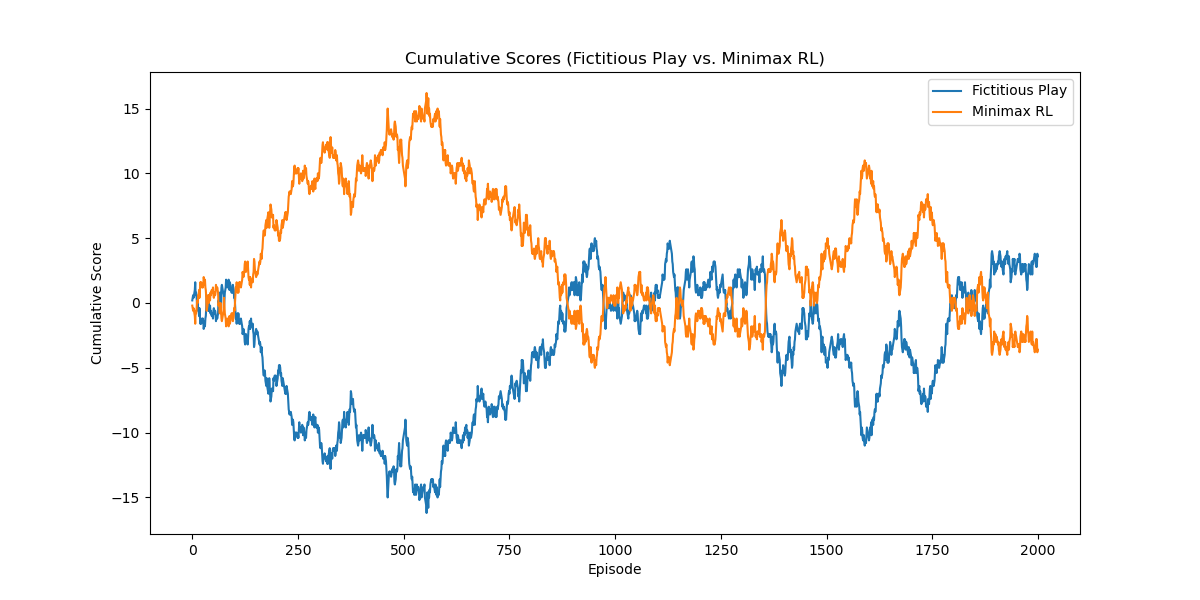
\includegraphics[width=0.6\textwidth]{mp-plots/fp_vs_mm_cumulative.png}
    \caption{Minimax RL vs.\ Fictitious Play hover around 
    zero.}
    \label{fig:mp-fp-mm-cumulative}
\end{figure}

\subsection{Overall Observations}

\begin{itemize}
    \item \textbf{Minimax RL} leverages the zero-sum nature of these 
    games, converging quickly to near-equilibrium policies. 
    \item \textbf{Q-Learning} exhibits persistent variability because 
    it views the opponent as part of a non-stationary environment, 
    preventing stable convergence in many runs.
    \item \textbf{Fictitious Play} and \textbf{Belief-Based} can do 
    well if the opponent is sufficiently predictable; otherwise, they 
    may remain off-equilibrium and be exploited by more adaptive 
    strategies.
    \item When both agents effectively randomize near equilibrium 
    (1/3 each in RPS or 1/2 each in MP), \emph{expected} cumulative 
    scores hover around zero. 
    \item Large divergences in cumulative scores generally mean one 
    agent discovered and exploited the other's systematic bias.
\end{itemize}

In summary, these plots confirm that specialized approaches like Minimax 
RL quickly home in on robust mixed strategies in strictly competitive 
games, while Q-Learning’s standard update rule struggles with the 
non-stationarity introduced by another learning opponent. Agents like 
Fictitious Play or Belief-Based may do quite well against certain 
opponents but can be exploited if they fail to adapt to changing 
opponent distributions.

\end{document}
